\section{Methods}
\label{hptpcPaper:sec:Methods}
\begin{itemize}
    \item Discussion of experimental setup
\item Beamline
\item Beam Instrumentation
\item UsToF
\item DsToF
    \begin{itemize}
        \item Description of the DsToF scintillator and bar configuration 
        \item Brief outline of the DsToF DAQ system
        \item DsToF efficiencies with appropriate plot
    \end{itemize}

\item (Cursory) TPC description
\item MC overview
\item Analysis methods and supporting plots; examples of ToF plots, proton and pion peaks with MC

\end{itemize}
    \subsection{CERN Beam Test}
    The beam test took place in the 0.8~GeV T10 beam line, East Area at the Proton Synchrotron in CERN from the 15th August to the 18th September 2018.
    The primary experimental setup for the data taking period is shown in figure~\ref{fig:setup}.
    \begin{figure}
    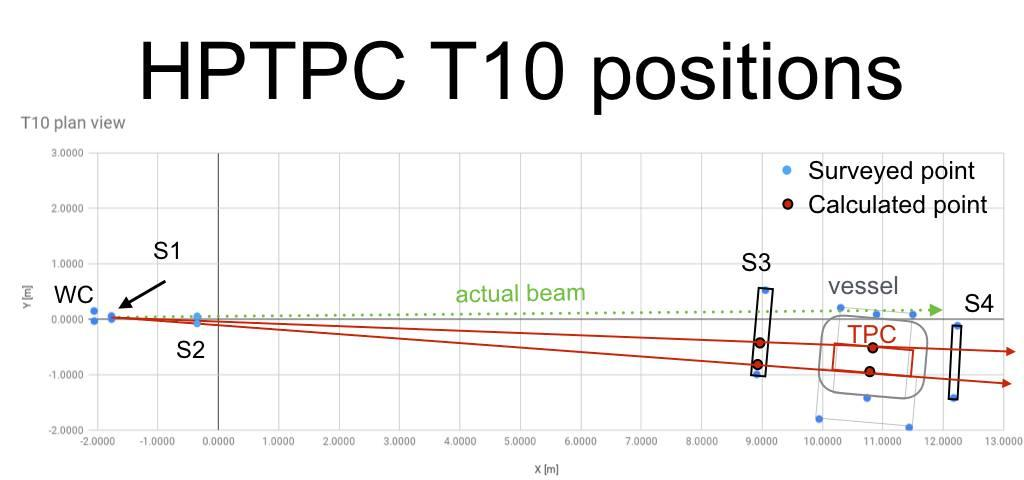
\includegraphics[width=1.0\linewidth]{files/Figures/T10Diagram.jpg}
    	\caption{Beam test configuration}
    		\label{fig:setup}
    \end{figure}
    The centre of the HPTPC Prototype was placed 13~m from the wire chamber at the beam entrance. 
    3 Time of Flight constituents, labeled S1 to S3, were placed upstream of the TPC, while the 4th, labeled S4, was placed directly downstream.
    Both the TPC and Time of Flight systems were placed at an off axis angle with resepct to the direction shown by the green arrow.
    Additionally, a variable number of blocks of acrylic moderator, shown in Figure~\ref{fig:modblocks}, were placed in the beamline, upstream of S1.
      \begin{figure}
      \centering
    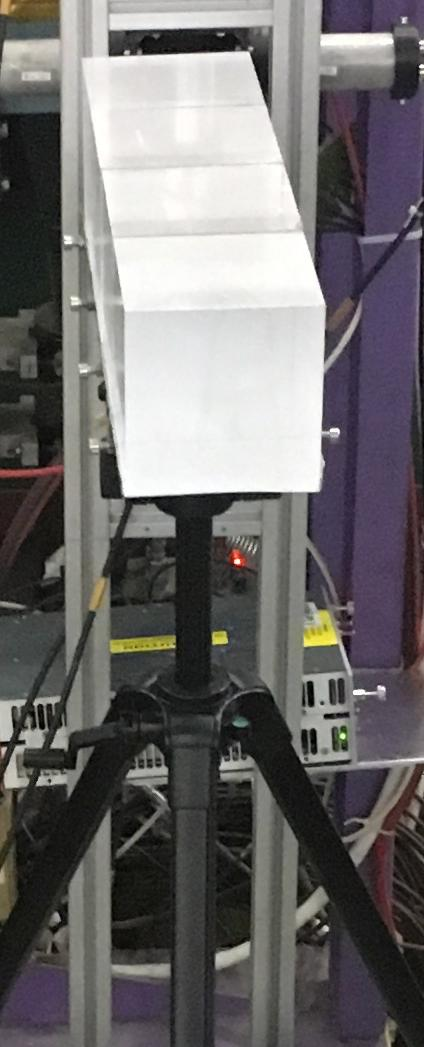
\includegraphics[width=0.2\linewidth]{files/Figures/ModeratorBlocks.jpg}
    	\caption{Acrylic Moderator Blocks}
    		\label{fig:modblocks}
    \end{figure}
    
    Moderator blocks were used in order to cause a spread in the incoming beam.
    The blocks cause protons to be spread through a larger angle than pions and other MIPs, increasing the off-axis proton pion ratio.
    The effect of this, together with placing the TPC and ToF systems off axis was to allow a measurement of protons with a lower pion background.
    This technique also had the effect of reducing the average momentum of the measured particles.
    Data were taken for 0, 1, 2, 3, and 4 moderator blocks in turn.
    
 
    
	\subsection{Upstream Time of Flight instrumentation (S1-3)}
    The upstream time of flight system was composed of the following constituents:
    S1 and S2, a 4~cm by 4~cm plastic counter with 30~ps resolution and a trigger counter resepctively. 
    S

	\subsection{Downstream Time of Flight instrumentation (S4)}
	
    The downstream time of flight system, S4, consists of 10 bars of Nuvia plastic scintillator, which form the detector medium. Attached to either end of each of these scintillator bars is a 5" Hamamatsu R6594 photomultiplier tube. The bars are arranged in two rows of five, such that there is complete coverage for any beam particles incident upon the detector. Diagrams of the S4 wall, along with its dimensions are presented in figure~\ref{fig:dstofFront} and~\ref{fig:dstofDiagonal}.
    
    The time resolution of the bars and PMTs was measured to be 1~ns. The spatial resolution of the bars and PMTs was measured to be 8.3~cm.
    
    \begin{figure}[ht]    
    	\begin{minipage}[t]{.48\textwidth}
    		\centering
    		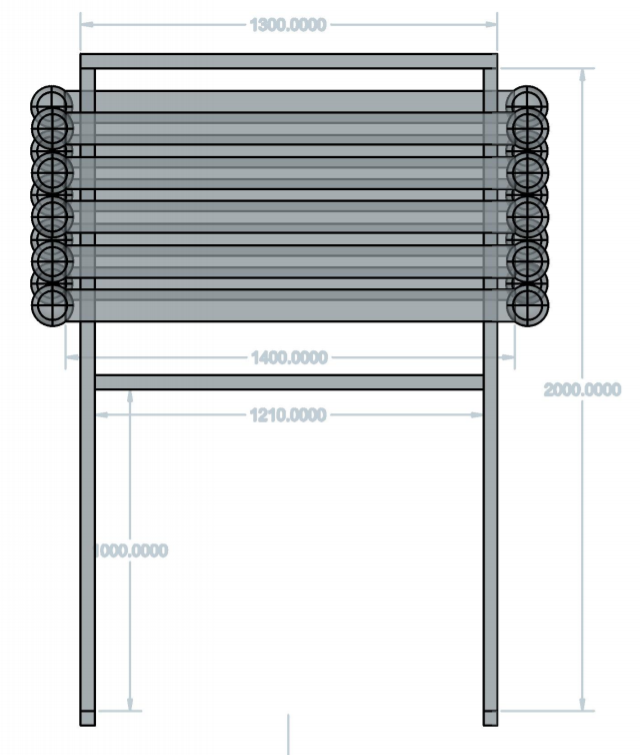
\includegraphics[width=0.6\linewidth]{files/Figures/dstofFront.png}
    		\caption{Front view of the downstream time of flight system}
    		\label{fig:dstofFront}
    	\end{minipage}
    	\hspace{0.3cm}
    	\begin{minipage}[t]{.48\textwidth}
    		\centering
    		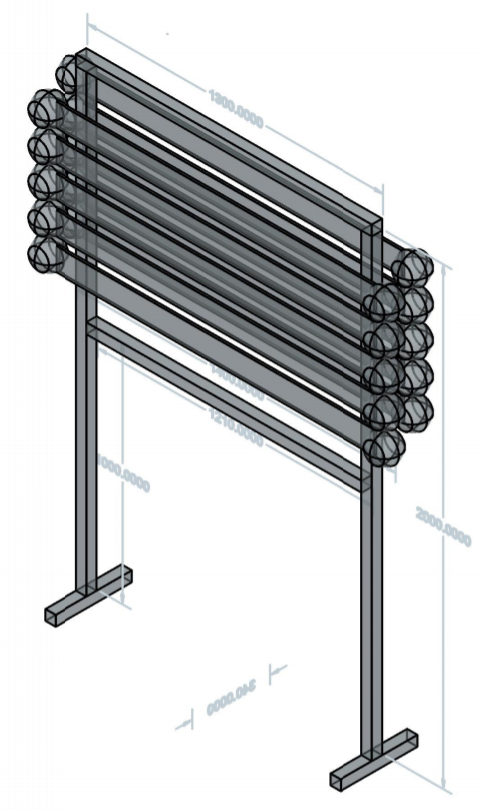
\includegraphics[width=0.45\linewidth]{files/Figures/dstofDiag.png}
    		\caption{Diagonal view of the downstream time of flight system showing more clearly the two rows of scintillator bars and photomultiplier tubes}
    		\label{fig:dstofDiagonal}
    	\end{minipage}
    \end{figure}
    
    All 20 of the photomultiplier tubes have their anode signals read out using NIM discriminators which are then fed into a time-to-digital converter. 
    
    A signal (i.e. an incident particle of any kind) in S4 was considered to have occurred if a signal was seen in both photomultiplier tubes on the same bar within 20~ns of each other.
    
    Additionally, a signal was also fed into the same time-to-digital converter whenever there was a coincidence between the S1 and S2 timing points. When calculating the time of flight of a given particle, this time of coincidence was used as first timing point.
    
	\subsection{Analysis methods -- $S_{4}$}

	Figure~\ref{fig:s4tof} shows the variation in the time of flight spectrum as recorded by the DsToF with a changing number of moderator blocks. This spectrum is formed from taking the difference in time between a coincidence being observed in the $S1$ and $S2$ timing points and a signal being recorded in $S4$ (the definition of an $S4$ signal is given above).
	
	\begin{figure}[h]
		\centering
		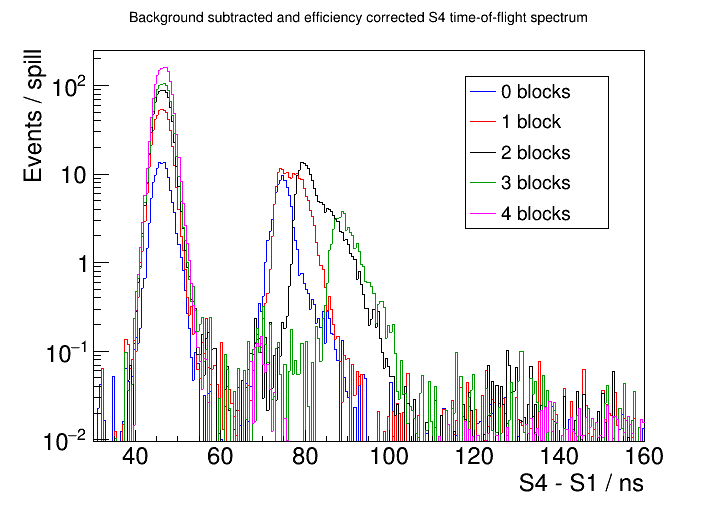
\includegraphics[width=0.7\linewidth]{files/Figures/s4ToF_axisAdj.png}
		\caption{$S_{4}$ time-of-flight spectra for varying numbers of moderator blocks. For all configurations, an exponentially falling background has been fitted and subtracted from the data. Additionally, the plot has also been corrected for the differing efficiencies of the various bars.}
		\label{fig:s4tof}	
	\end{figure}

	Furthermore, two corrections are applied to this measurement to give fig.~\ref{fig:s4tof}. Timing delays caused by cabling and equipment have to be taken into account. For this, a Gaussian is fitted to the peak caused by quicker particles and the mean of this is treated to have a value of $S4 - S1$ which corresponds to a particle traversing the distance between $S1$ and $S4$ at the speed of light. The other times are then shifted by the same amount.
	
	Additionally, the measurements are adjusted for the efficiency of each bar. The efficiency of each bar is calculated by taking the number of signal hits in coincidence with an $S1-S2$ signal in each bar and dividing by the total number of PMT hits in each bar which are themselves in coincidence with an $S1-S2$ signal. If we express the number of single PMT hits which are in coincidence with $S1-S2$ signal as $N_{1PMTcoins}$ and the number of 2 PMT signals in coincidence with an $S1-S2$ signal as $N_{2PMTcoins}$ then the efficiency is given by~(\ref{eq:barEff}).
	
	\begin{equation}
		\epsilon = \frac{N_{2PMTcoins}}{N_{2PMTcoins}+N_{1PMTcoins}}
		\label{eq:barEff}
	\end{equation}
	
	Using fig.~\ref{fig:s4tof} protons and MIPs are selected with timing cuts. These timing cuts are chosen by fitting a sum of signal and background functions to the time-of-flight spectra shown in figure~\ref{fig:s4tof}. The signal functions are taken to be Gaussians while the background is taken to be an exponential function. An example of this is shown in figure~\ref{fig:fitEx}.
	
	\begin{figure}[h]
		\centering
		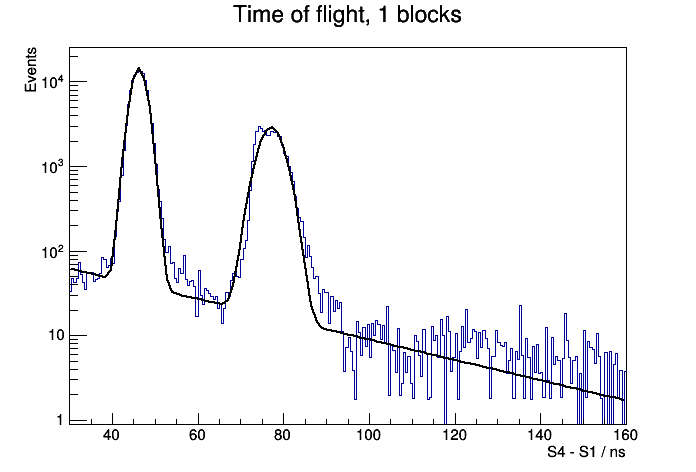
\includegraphics[width=0.6\textwidth]{files/Figures/1_dtof1d}
		\caption{Example of the time-of-flight spectrum observed in $S4$ with a combined signal and background function fitted (shown in black)}
		\label{fig:fitEx}
	\end{figure}

	To produce the data used in this analysis, an exponential background function is subtracted. The parameters for this function are taken from the combined signal and background function.
	
	\subsection{Analysis methods -- $S3$}
	
	
	\begin{figure}[h]
		\centering
		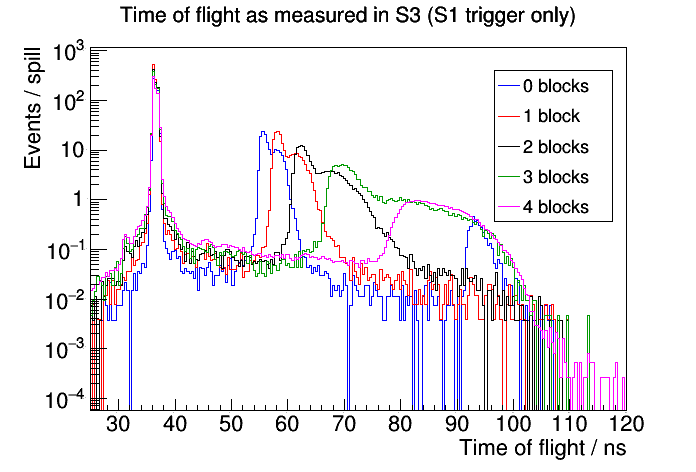
\includegraphics[width=0.6\textwidth]{files/Figures/utof1dS1Log}
	\end{figure}
	